\renewcommand{\thispart}{5 }
\renewcommand{\thispartname}{Practical Issues in Neural Network Training}

\part{\thispartname}

% Cover page
\section{Outline}
%
% Cover page for giveb part
%

\title[\modulename - Part \thispart]
{
  {\bf 
   \modulename - 
   Part \thispart\\
  }
  \vspace{0.5cm}
  {\it 
   \color{yellow}
    \secname\\
  }
}
\author[C.Andreopoulos] {
  Professor Costas Andreopoulos\inst{1,2}, {\it FHEA}
}
\institute[Liverpool/STFC-RAL] {
   \inst{1} University of Liverpool, Department of Physics\\
   \vspace{0.3cm}
   {\it {\color{magenta} Lectures delivered at the University of Liverpool, 2024-25}}\\
   \vspace{0.2cm}
}
\date{\today}

\titlegraphic{
  
\includegraphics[height=30px]{images/logo/liverpool.png}
}

\begin{frame}[plain]
  \titlepage
\end{frame}




% Outline
%
% Table of contents to be displayed at the beginning of each part
%

\begin{frame}[t,allowframebreaks]{Outline for Part \thispart -}
  % Part \thispart (\secname) covers the following topics:\\
  % \vspace{0.5cm}
  \linespread{1.1}
  \setcounter{secnumdepth}{3}
  \setcounter{tocdepth}{3}
  % \tableofcontents[currentsection, hideothersubsections, sectionstyle=hide/hide]
  \tableofcontents[part=\thispart]
\end{frame}



\section{Generalization}
\begin{frame}[t,allowframebreaks]{Generalization -}

    Training a \gls{ml} model {\em looks like} an optimization task.\\
    \vspace{0.1cm}
    \begin{blockexample}{}
      Typically, to train a \gls{ml} model: 
      \begin{itemize}
        \item 
        We use a \index{training set}\gls{training set} 
        that contains a number of examples, and
        \item
        define a \index{loss function}\gls{loss function},
        a measure of training error over that set.
      \end{itemize}
      The training process adjusts the model parameters
      to optimize the model performance (minimize the training error).\\
    \end{blockexample}
    \vspace{0.2cm}
    However, {\bf training a \gls{ml} model is not a pure optimization problem}.\\
    \vspace{0.2cm}
    Our \gls{ml} model should {\bf maintain a satisfactory performance 
    with new, previously unseen inputs} - 
    not just for the inputs in the training set.\\
    \vspace{0.2cm}
    Performing well for previously unseen inputs is called 
    \index{generalization}\gls{generalization}.\\
    \vspace{0.2cm}
    How to build model that generalize is one of the central problems in \gls{ml}.


    \framebreak

    %
    %

    In the linear regression example, our model
    \begin{equation}
        \hat{y} = {\mathbf x}^T \cdot {\mathbf w}
        %\label{eq:}
    \end{equation}        

    was trained using a set $\mathbb{D}$ of $N_{(train)}$
    training examples $({\mathbf x_{(train)}},y_{(train)})$, 
    by minimizing the loss function
    \begin{equation}
        L_{(train)} = \frac{1}{N_{(train)}} 
        \sum_{({\mathbf x_{(train)}},y_{(train)})  \in \mathbb{D}}
        \Big( y_{(train)} - {\mathbf x_{(train)}}^T \cdot {\mathbf w} \Big)^2
        %\label{eq:}
    \end{equation}        

    However, we care for the test error
    \begin{equation}
        L_{(test)} = \frac{1}{N_{(test)}} 
        \sum_{({\mathbf x_{(test)}},y_{(test)})  \in \mathbb{T}}
        \Big( y_{(test)} - {\mathbf x_{(test)}}^T \cdot {\mathbf w} \Big)^2
        %\label{eq:}
    \end{equation}        
    for the $N_{(test)}$ test examples $({\mathbf x_{(test)}},y_{(test)})$ 
    of the set $\mathbb{T}$.

    \framebreak

    %
    %

    What can we say about the \gls{ml} model performance on the test set,
    if we only ever see the training set?
    \begin{itemize}
        \item
        Not much, unless the test and training data sets come from the 
        {\bf same data-generating process}.    
    \end{itemize}
    \vspace{0.2cm}   
    Typically, we make assumptions known as the {\bf i.i.d. assumptions}.\\
    \vspace{0.2cm}
    The examples in the test and training sets are assumed to be:
    \begin{itemize}
        \item {\bf independent}, and
        \item {\bf identically distributed}, 
        i.e. they are drawn from the same probability distribution 
        (the data-generating distribution)
    \end{itemize}
    \vspace{0.2cm}
    With the i.i.d assumptions:
    \begin{itemize}
        \item
        we can describe the data-generating process
        with a probability distribution over a single data example, and
        \item
        study the relationship between the training and test error.
    \end{itemize}

\end{frame}


\section{Capacity, overfitting and underfitting}


\begin{frame}[t,allowframebreaks]{Underfitting and overfitting -}

    Typically, 
    we we choose model parameters that reduce the training error, 
    and then test the model performance against the test set.
    \begin{itemize}
    \item 
    Under this process, 
    the expected value of the test error 
    is greater than (or equal to)  
    the expected value of the training error.
    \end{itemize}
 
    \vspace{0.2cm}
    
    A central challenge is to:
    \begin{itemize}
     \item {\bf reduce the training error}, \underline{and}
     \item {\bf reduce the gap between the training and test error}.
    \end{itemize}
 
    \vspace{0.2cm}   
 
    Failing on either of these goals, gives rise to common model pathologies:
    \begin{itemize}
      \item \index{underfitting}\Gls{underfitting}:
      Our model does not describe the training data well,
      and {\bf we cannot obtain a sufficiently small training error}.
      \item \index{overfitting}\Gls{overfitting}:
      We obtain a small training error,
      but {\bf our model does not generalize well} and  
      the training error is large. 
    \end{itemize}
 
    \framebreak
 
    %
    %
 
    \begin{center}
         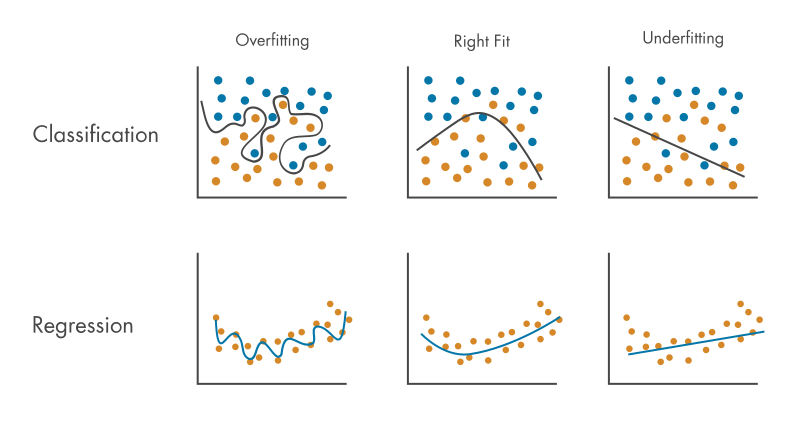
\includegraphics[width=1.0\textwidth]
             {./images/training_issues/over_and_underfitting_1.png}\\
         {\tiny 
             Illustrating overfitted and underfitted model pathologies.\\
             \color{col:attribution} 
             Schematic reproduced from \cite{MathWorks:Overfitting}.\\
         }
     \end{center}
 
 \end{frame}
 

\begin{frame}[t,allowframebreaks]{Capacity -}

    We can affect the tendency of a \gls{ml} model for 
    \index{underfitting}\gls{underfitting} or 
    \index{overfitting}\gls{overfitting},
    by adjusting its 
    \index{capacity}\gls{capacity}.\\

    \vspace{0.2cm}

    The \gls{capacity} of a model is its 
    {\bf ability to describe a broad variety of data-generating processes}.

    \vspace{0.2cm}

    \begin{itemize}
        \item 
        {\bf Models with low capacity, 
        will struggle capturing all the details} 
        of the training data and providing a satisfactory fit.\\
        % \begin{blockexample}{}
        %     \small
        %     For example, imagine using a linear model $\hat{y} = b+wx$
        %     to fit data sampled from a data-generating process with a 
        %     probability distribution that is quadratic in $x$.
        % \end{blockexample}
        \item 
        {\bf Models with high capacity 
        can memorize unimportant features} of the data
        that do not serve the purpose of model generalization.
        % \begin{blockexample}{}
        %     \small
        %     For example, imagine using a 10$^{th}$ order polynomial to
        %     to fit noisy data sampled from a data-generating process with a 
        %     probability distribution that is linear in $x$.
        % \end{blockexample}
    \end{itemize}

    \vspace{0.2cm}

    Occam's razor (the `law of parsimony')
    \cite{Wikipedia:OccamRazor} is a good guiding principle:
    Amongst competing hypotheses that describe the data equally well,
    chose the simples one.\\

    \vspace{0.2cm}

    While simpler models are likely to generalize better,
    we still need a sufficiently complex model to achieve low training error.

    \framebreak

    %
    %

    A central task in \gls{ml} is to {\bf match the capacity of the model
    to the complexity of its task and to the amount of available data.}\\

    \vspace{0.1cm}

    \begin{center}
        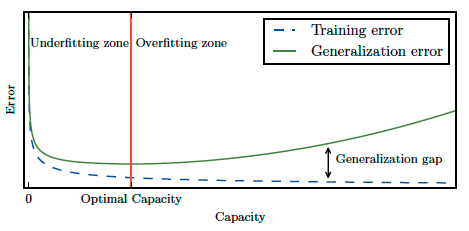
\includegraphics[width=0.90\textwidth]
            {./images/training_issues/error_vs_capacity_1.png}\\
        {\tiny 
            Illustrating the relationship between error and capacity.\\
            \color{col:attribution} 
            Schematic reproduced from p. 112 of \cite{Goodfellow:2017MITDL}.\\
        }
    \end{center}

    \framebreak

    %
    %

    There are several ways to affect the capacity of a model.


\end{frame}


\section{No free lunch theorem}

\begin{frame}[t]{The `no free lunch' theorem}

Can we really infer general rules from a finite set of training examples?
\begin{itemize}
  \item Inductive reasoning is {\bf intrinsically uncertain}.
  \item \gls{ml} does not offer any rule with certainty - 
  only rules that are {\bf {\em probably} correct for {\em most} input data examples}.
\end{itemize}

\vspace{0.1cm}

\begin{blockexample}{}
\underline{The `{\bf no free lunch theorem}' of  \gls{ml}} 
by D.Wolpert and W.Macready \cite{NoFreeLunch}.\\
\vspace{0.2cm}
{\small
Averaged over all data-generating distributions,
every classification algorithm has the same generalisation performance
against previously unseen examples.\\
}
\end{blockexample}

\vspace{0.1cm}

The `no free lunch theorem' implies there is 
{\bf no universal learning algorithm} 
performing well for all possible data-generating distributions.

\vspace{0.2cm}

However, by building in some assumptions,
{\bf we can design algorithms that work well in specific real-world application}.

\end{frame}


\section{Vanishing and exploding gradient problems}
%  - Leaky ReLU and maxout 

\section{Difficulties in convergence}
\section{Local optima}
\section{Bias-variance trade-off}
\section{Regularization methods for deep learning}

\begin{frame}[t,allowframebreaks]{Regularization -}

\end{frame}

\subsection{Norm penalties: L2 and L1 regularization}
\subsection{Dataset augmentation}
\subsection{Noise robustness}
\subsection{Multitask learning}
\subsection{Early stopping}
\subsection{Parameter sharing}
\subsection{Ensemble methods: Bagging, subsampling and dropout}
\subsection{Adversarial Training}


% Suggested reading for this part
\section{Suggested reading}
%
%
%

\begin{frame}{Suggested reading for Part \thispart}

    {
        \small
        Essential reading on {\bf automatic differentiation}:
        \begin{itemize}
            \scriptsize
            \item Section 6.5 from the `Deep Learning' 
            textbook of Goodfellow, Bengio and Courville \cite{Goodfellow:2017MITDL}.
            \item Appendix B from the `Machine Learning Refined' 
            textbook of Watt, Borhani and Katsaggelos \cite{Watt:2016Cambridge}.
            \item `A review of automatic differentiation and its 
            efficient implementation' by Margossian \cite{Margossian:2019ad}
        \end{itemize}
        
        Also, you may want to browse:
        \begin{itemize}
            \scriptsize
            \item The collection of articles
             in the book `Automatic Differentiation: Applications, Theory, and Implementations'
             edited by B{\"u}cker, Corliss, Hovland, Naumann and Norris \cite{Bucker:2005ABo}
        \end{itemize}
    }
    

\end{frame}
